\documentclass{standalone}

\usepackage{tikz}

\begin{document}

  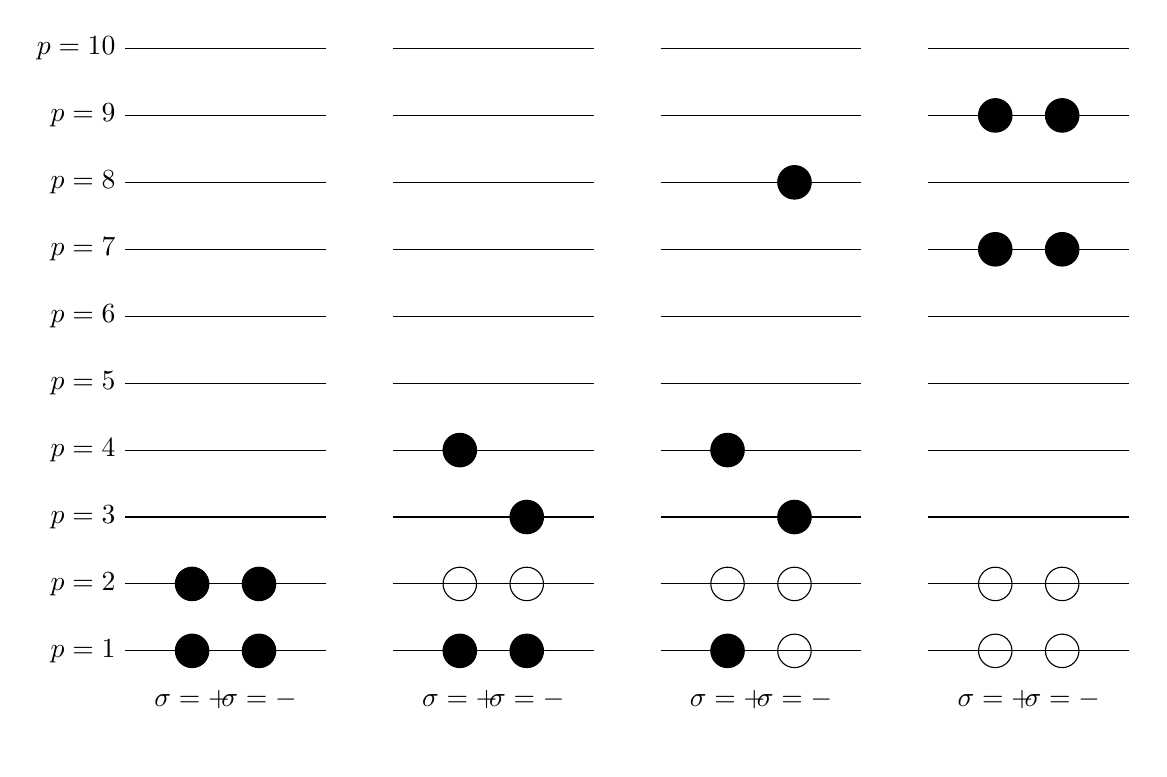
\begin{tikzpicture}[scale=0.85]
    \begin{scope}
      \foreach \i in {1,...,10}
      {
        \draw (-1,\i-1) node[anchor=east] {$p = \i$} --(2,\i-1);
      }
      \filldraw (0,0) node[anchor=north,inner sep=.5cm] {$\sigma=+$} circle (0.25cm); \filldraw (1,0) node[anchor=north,inner sep=.5cm] {$\sigma=-$} circle (0.25cm);
      \filldraw (0,1) circle (0.25cm); \filldraw (1,1) circle (0.25cm);
    \end{scope}
    \begin{scope}[xshift=4cm]
      \foreach \i in {1,...,10}
      {
        \draw (-1,\i-1) --(2,\i-1);
      }
      \filldraw (0,0) node[anchor=north,inner sep=.5cm] {$\sigma=+$} circle (0.25cm); \filldraw (1,0) node[anchor=north,inner sep=.5cm] {$\sigma=-$} circle (0.25cm);
      \draw (0,1) circle (0.25cm); \draw (1,1) circle (0.25cm);
      \filldraw (0,3) circle (0.25cm); \filldraw (1,2) circle (0.25cm);
    \end{scope}
    \begin{scope}[xshift=8cm]
      \foreach \i in {1,...,10}
      {
        \draw (-1,\i-1) --(2,\i-1);
      }
      \filldraw (0,0) node[anchor=north,inner sep=.5cm] {$\sigma=+$} circle (0.25cm); \draw (1,0) node[anchor=north,inner sep=.5cm] {$\sigma=-$} circle (0.25cm);
      \draw (0,1) circle (0.25cm); \draw (1,1) circle (0.25cm);
      \filldraw (0,3) circle (0.25cm); \filldraw (1,2) circle (0.25cm);
      \filldraw (1,7) circle (0.25cm); 
    \end{scope}
    \begin{scope}[xshift=12cm]
      \foreach \i in {1,...,10}
      {
        \draw (-1,\i-1) --(2,\i-1);
      }
      \draw (0,0) node[anchor=north,inner sep=.5cm] {$\sigma=+$} circle (0.25cm); 
      \draw (1,0) node[anchor=north,inner sep=.5cm] {$\sigma=-$} circle (0.25cm);
      \draw (0,1) circle (0.25cm); 
      \draw (1,1) circle (0.25cm);
      \filldraw (0,6) circle (0.25cm); 
      \filldraw (1,6) circle (0.25cm);
      \filldraw (0,8) circle (0.25cm); 
      \filldraw (1,8) circle (0.25cm);
    \end{scope}

  \end{tikzpicture}

\end{document}